\documentclass[10pt]{beamer}

\usetheme{metropolis}
\usepackage{appendixnumberbeamer}
\usepackage{booktabs}
\usepackage[scale=2]{ccicons}
\usepackage{pgfplots}
\usepgfplotslibrary{dateplot}

\usepackage{xspace}
\newcommand{\themename}{\textbf{\textsc{metropolis}}\xspace}

\usepackage{graphicx}

\usepackage{tikz}
\usetikzlibrary{positioning,arrows,shapes}
\pgfplotsset{compat=1.18}


\metroset{titleformat=smallcaps,numbering=fraction}

\title{Policy Conflicts and Strategies in the Policy-Making Process}
\subtitle{POSC 315: Introduction to Public Policy}
\date{\today}
\author{David P. Adams, Ph.D.}
\institute{California State University, Fullerton}

\begin{document}

\maketitle

\begin{frame}{Table of contents}
 \setbeamertemplate{section in toc}[sections numbered]
 \tableofcontents[hideallsubsections]
\end{frame}

\section{Learning Objectives}

\begin{frame}
\frametitle{Learning Objectives}
\begin{itemize}
   \item Understand the \alert{sources} of policy conflict.
   \item Explore \alert{strategies} to manage or resolve policy conflicts.
   \item Reflect on how conflict can serve as both a \alert{challenge} and an \alert{opportunity}.
   \item Develop a foundation for applying these concepts to \alert{real-world policy issues}.
\end{itemize}

\begin{figure}
   \centering
   \begin{tikzpicture}
       \node[draw, circle, minimum size=1.5cm] (sources) {
\includegraphics[width=1cm]{images/handshake.jpeg}};
       \node[draw, circle, minimum size=1.5cm, right of=sources, xshift=2cm] (strategies) {
\includegraphics[width=1cm]{images/scales-of-justice.jpeg}};
       \node[draw, circle, minimum size=1.5cm, right of=strategies, xshift=2cm] (challenge-opportunity) {
\includegraphics[width=1cm]{images/lightbulb.png}};
       \node[draw, circle, minimum size=1.5cm, right of=challenge-opportunity, xshift=2cm] (real-world) {
\includegraphics[width=1cm]{images/skyline.jpeg}};
   \end{tikzpicture}
   \caption{Learning Objectives}
\end{figure}
\end{frame}

\section{What is Policy Conflict?}

\begin{frame}
\frametitle{What is Policy Conflict?}
\begin{itemize}
   \item \textbf{Definition:} A situation where stakeholders have \alert{opposing interests, goals, or values}.
   \item \textbf{Key Elements:}
       \begin{itemize}
           \item \textbf{Competing Interests:} Economic vs. environmental priorities.
           \item \textbf{Value Clashes:} Individual rights vs. collective welfare.
           \item \textbf{Limited Resources:} Funding, time, or personnel.
       \end{itemize}
\end{itemize}

\begin{figure}
   \centering
   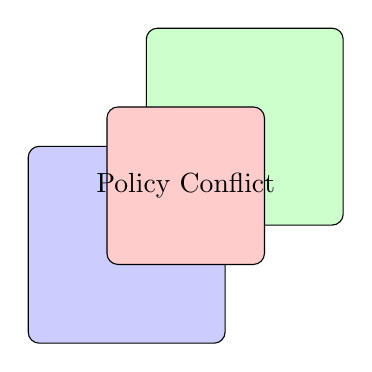
\begin{tikzpicture}[scale=0.5]
       \draw[fill=blue!20, rounded corners] (0,0) rectangle (5,5);
       \draw[fill=green!20, rounded corners] (3,3) rectangle (8,8);
       \draw[fill=red!20, rounded corners] (2,2) rectangle (6,6);
       \node at (4,4) {Policy Conflict};
   \end{tikzpicture}
   \caption{Elements of Policy Conflict}
\end{figure}
\end{frame}

\begin{frame}
\frametitle{Common Sources of Conflict}
\begin{enumerate}
   \item \textbf{Differing Stakeholder Interests:}
       \begin{itemize}
           \item Example: Businesses prioritize profits; activists prioritize sustainability.
       \end{itemize}
   \item \textbf{Ideological Differences:}
       \begin{itemize}
           \item Example: Debates over government intervention in healthcare.
       \end{itemize}
   \item \textbf{Resource Limitations:}
       \begin{itemize}
           \item Limited budgets often spark competition for allocation.
       \end{itemize}
   \item \textbf{Regulatory Constraints:}
       \begin{itemize}
           \item Federal vs. state jurisdiction conflicts.
       \end{itemize}
\end{enumerate}

\begin{figure}
   \centering
   \begin{tikzpicture}[scale=0.8]
       \node[draw, circle, minimum size=1.5cm] (interests) {
\includegraphics[width=1cm]{images/briefcase.png}};
       \node[draw, circle, minimum size=1.5cm, right of=interests, xshift=2cm] (ideology) {
\includegraphics[width=1cm]{images/debate.png}};
       \node[draw, circle, minimum size=1.5cm, right of=ideology, xshift=2cm] (resources) {
\includegraphics[width=1cm]{images/money-bag.png}};
       \node[draw, circle, minimum size=1.5cm, right of=resources, xshift=2cm] (regulations) {
\includegraphics[width=1cm]{images/gavel.png}};
   \end{tikzpicture}
   \caption{Sources of Policy Conflict}
\end{figure}
\end{frame}

\begin{frame}
\frametitle{Stakeholder Interest Conflicts}
\begin{columns}[T,onlytextwidth]
   \column{0.5\textwidth}
   \begin{block}{Environmental Policy Example}
       \begin{itemize}
           \item \textbf{Conflict:} Economic development vs. conservation.
           \item \textbf{Stakeholders:} Industry, environmental groups, local communities.
       \end{itemize}
   \end{block}
   \column{0.5\textwidth}
   \begin{block}{Social Policy Example}
       \begin{itemize}
           \item \textbf{Conflict:} Equity vs. efficiency in welfare programs.
           \item \textbf{Stakeholders:} Taxpayers, beneficiaries, policymakers.
       \end{itemize}
   \end{block}
\end{columns}

\begin{figure}
   \centering
   \begin{tikzpicture}
       \node[draw, circle, minimum size=2cm] (factory) {
\includegraphics[width=1.5cm]{images/factory.png}};
       \node[draw, circle, minimum size=2cm, right of=factory, xshift=3cm] (forest) {
\includegraphics[width=1.5cm]{images/forest.png}};
   \end{tikzpicture}
   \caption{Stakeholder Interest Conflicts}
\end{figure}
\end{frame}

\begin{frame}
   \frametitle{Ideological Clashes in Policy}
   \begin{itemize}
       \item Examples of Ideological Conflicts:
           \begin{enumerate}
               \item \textbf{Healthcare Reform:} Individual responsibility vs. collective welfare.
               \item \textbf{Tax Policies:} Redistribution vs. growth-oriented strategies.
           \end{enumerate}
       \item \textbf{Impact:}
           \begin{itemize}
               \item Polarized debates slow policymaking processes.
           \end{itemize}
   \end{itemize}
   
   \begin{figure}
       \centering
       \begin{tikzpicture}
           \begin{axis}[
               width=0.8\textwidth,
               height=0.5\textwidth,
               mbarplot,
               xlabel={Year},
               ylabel={Ideological Divide},
               xtick={2010, 2012, 2014, 2016, 2018, 2020},
               xticklabels={2010, 2012, 2014, 2016, 2018, 2020},
               legend pos=north west
           ]
           \addplot plot coordinates {(2010, 65) (2012, 70) (2014, 75) (2016, 80) (2018, 85) (2020, 90)};
           \addplot plot coordinates {(2010, 60) (2012, 65) (2014, 70) (2016, 75) (2018, 80) (2020, 85)};
           \legend{House, Senate}
           \end{axis}
       \end{tikzpicture}
       \caption{Ideological Divide in U.S. Congress Over Time}
   \end{figure}
\end{frame}
   

\begin{frame}
   \frametitle{Limited Resources as a Conflict Source}
   \begin{itemize}
       \item \textbf{Definition:} Insufficient resources create competition among stakeholders.
       \item Examples:
       \begin{enumerate}
           \item \textbf{Infrastructure Funding:} Which projects get priority?
           \item \textbf{Disaster Relief Allocation:} Balancing urgency and equity.
       \end{enumerate}
       \item \textbf{Outcome:} Resource constraints often lead to incremental decisions.
   \end{itemize}
   
   \vspace{0.3cm} % Adjust spacing here if needed

   \begin{figure}
       \centering
       \resizebox{0.75\textwidth}{!}{% Scale the tikz figure
           \begin{tikzpicture}
               \pie[
                   text depth=0.2em, % Smaller text depth
                   title=Government Budget Allocation,
                   fontsize=\scriptsize, % Smaller font size
                   radius=1.5, % Smaller radius
                   color={blue!60, red!60, green!60, yellow!60}
               ]{
                   40/Defense,
                   30/Healthcare,
                   20/Education,
                   10/Other
               }
           \end{tikzpicture}
       }
       \caption{\scriptsize Government Budget Allocation} % Smaller caption size
   \end{figure}
\end{frame}

   
\begin{frame}
   \frametitle{Bureaucratic and Regulatory Barriers}
   \begin{itemize}
       \item \textbf{Definition:} Conflicts arising from overlapping or restrictive regulations.
       \item Example:
           \begin{itemize}
               \item Federal vs. state laws on marijuana legalization.
           \end{itemize}
       \item \textbf{Impact on Policymaking:}
           \begin{itemize}
               \item Delayed implementation.
               \item Increased litigation costs.
           \end{itemize}
   \end{itemize}
   
            

   
   \end{itemize}
   
   \begin{figure}
       \centering
       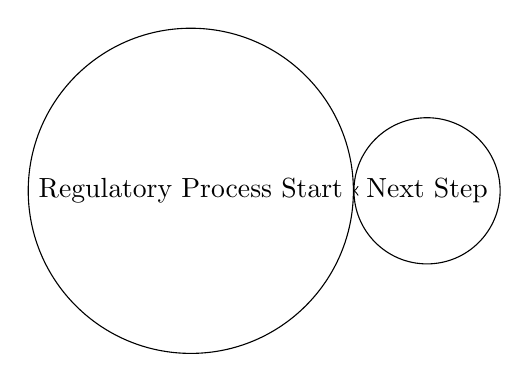
\begin{tikzpicture}
           \node[draw, circle, minimum size=1.5cm] (start) {Regulatory Process Start};
           \node[draw, circle, minimum size=1.5cm, right of=start, xshift=2cm] (next) {Next Step};
           \draw[->] (start) -- (next);
       \end{tikzpicture}
       \caption{Regulatory Process Diagram}
   \end{figure}
   
   \section{Managing Policy Conflicts}

   \begin{frame}
   \frametitle{Managing Policy Conflicts}
   \begin{itemize}
       \item \textbf{Key Strategies:}
           \begin{enumerate}
               \item \textbf{Negotiation:} Direct discussions for compromise.
               \item \textbf{Mediation:} Third-party facilitation.
               \item \textbf{Collaboration:} Joint decision-making.
               \item \textbf{Litigation:} Resolving disputes through courts.
           \end{enumerate}
       \item \textbf{Importance:} Effective management ensures progress and stakeholder satisfaction.
   \end{itemize}
   \end{frame}
   
   \begin{frame}
   \frametitle{Negotiation as a Strategy}
   \begin{itemize}
       \item \textbf{Definition:} Direct discussions among stakeholders to reach a compromise.
       \item \textbf{Advantages:}
           \begin{itemize}
               \item Cost-effective.
               \item Builds relationships.
           \end{itemize}
       \item \textbf{Challenges:}
           \begin{itemize}
               \item Power imbalances.
               \item Requires trust and communication.
           \end{itemize}
       \item \textbf{Real-World Example:} U.S. budget negotiations between Congress and the President.
   \end{itemize}
   \end{frame}

\end{document}